% !TEX TS-program = pdflatex
% !TEX encoding = UTF-8 Unicode

% This is a simple template for a LaTeX document using the "article" class.
% See "book", "report", "letter" for other types of document.

% TODO: Ich habe eventuell irgendwo geschrieben, dass in Haskell kein Ad-Hoc-Polymorphismus benutzt
% wird, was ja Quatsch ist, da das ja gerade der Zweck von Typklassen ist.

\documentclass[11pt]{article} % use larger type; default would be 10pt

\usepackage[utf8]{inputenc} % set input encoding (not needed with XeLaTeX)

\usepackage{todonotes}
\usepackage{mathrsfs}
\usepackage{graphicx}
\usepackage{minted}

%%% Examples of Article customizations
% These packages are optional, depending whether you want the features they provide.
% See the LaTeX Companion or other references for full information.

%%% PAGE DIMENSIONS
\usepackage{geometry} % to change the page dimensions
\geometry{a4paper} % or letterpaper (US) or a5paper or....
% \geometry{margin=2in} % for example, change the margins to 2 inches all round
% \geometry{landscape} % set up the page for landscape
%   read geometry.pdf for detailed page layout information

\usepackage{graphicx} % support the \includegraphics command and options

\usepackage{courier}
\usepackage{amsmath}

\usepackage[ngerman]{babel}

% \usepackage[parfill]{parskip} % Activate to begin paragraphs with an empty line rather than an indent

%%% PACKAGES
\usepackage{booktabs} % for much better looking tables
\usepackage{array} % for better arrays (eg matrices) in maths
\usepackage{paralist} % very flexible & customisable lists (eg. enumerate/itemize, etc.)
\usepackage{verbatim} % adds environment for commenting out blocks of text & for better verbatim
\usepackage{subfig} % make it possible to include more than one captioned figure/table in a single float
% These packages are all incorporated in the memoir class to one degree or another...

\usepackage{amssymb}

%%% HEADERS & FOOTERS
\usepackage{fancyhdr} % This should be set AFTER setting up the page geometry
\pagestyle{fancy} % options: empty , plain , fancy
\renewcommand{\headrulewidth}{0pt} % customise the layout...
\lhead{}\chead{}\rhead{}
\lfoot{}\cfoot{\thepage}\rfoot{}

%%% SECTION TITLE APPEARANCE
\usepackage{sectsty}
\allsectionsfont{\sffamily\mdseries\upshape} % (See the fntguide.pdf for font help)
% (This matches ConTeXt defaults)

%%% ToC (table of contents) APPEARANCE
\usepackage[nottoc,notlof,notlot]{tocbibind} % Put the bibliography in the ToC
\usepackage[titles,subfigure]{tocloft} % Alter the style of the Table of Contents
\renewcommand{\cftsecfont}{\rmfamily\mdseries\upshape}
\renewcommand{\cftsecpagefont}{\rmfamily\mdseries\upshape} % No bold!

%%% END Article customizations

%%% The "real" document content comes below...

\title{Anfang}
\author{Thomas Rossow}
%\date{} % Activate to display a given date or no date (if empty),
         % otherwise the current date is printed 

\begin{document}
\tableofcontents 
\maketitle

\section{Einleitung}

Die funktionale Programmiersprache Haskell bietet ein komplexes Typsystem, das auf der Typinferenz nach Hindley-Milner basiert \todo{cite}.
Zu jedem Ausdruck lässt sich eine Typsignatur herleiten, die den allgemeinsten Typen dieses Ausdrucks darstellt. Außerdem
kann der Programmierer zu jedem Ausdruck eine Typsignatur angeben, was zur Übersicht beiträgt und Fehlern vorbeugt.
Das Typsystem ist so mächtig, dass die Typsignatur allein schon sehr viele Rückschlüsse über die zugehörige Funktion ermöglicht.
Betrachten wir beispielhaft die folgende Signatur.

\begin{minted}{haskell}
test :: (a -> b) -> [a] -> [b]
\end{minted}

Allein durch diesen Typen lässt sich bereits erahnen, was sich ungefähr hinter dieser Funktion verbirgt. Die Funktion nimmt
eine Funktion und eine Liste als Argumente. Die Funktion muss dabei den Typen der Listenelemente auf einen anderen Typen
abbilden. Als Ergebnis liefert die Funktion den Rückgabetypen der übergebenen Funktion. Es ist anzunehmen, dass die Funktion
\texttt{test} die Eingabeliste mithilfe der übergebenen Funktion manipuliert und die resultierende Liste zurückgibt.

Haskell liefert eine solche Funktion in der Prelude, man kennt sie unter dem Namen \texttt{map}. Dass sich \texttt{test} und
\texttt{map} eine Typsignatur teilen, lässt also Rückschlüsse auf eine ähnliche Funktionsweise zu. Doch diese Ähnlichkeit
ist nicht auf vage Aussagen beschränkt, man kann ganz systematisch korrekte Aussagen zu beliebigen Typsignaturen
herleiten, wie \cite{xyz} \todo{cite} zeigt.

Die Herleitung freier Theoreme ist so generisch, dass sie auch programmtisch erledigt werden kann. Genau das macht
\cite{bla} \todo{cite} - hierbei handelt es sich um die Bibliothek \textit{free-theorems}, die es ermöglicht, Haskell-Code einzulesen
und aus beliebigen Typsignaturen Formeln zu generieren, die die entsprechenden freien Theoreme repräsentieren. Zudem gibt es
mit \cite{x} \todo{cite} eine Webanwendung, die einen Zugriff auf die Funktionen der Bibliothek ermöglicht.
Leider bietet die Bibliothek \textit{free-theorems} nicht sämtliche Sprachfunktionen von Haskell an. 

Ein wichtiger Aspekt
bei der Programmierung in Haskell sind Typklassen. Sie ermöglichen es, Datenstrukturen in Klassen einzuordnen, und für diese
Klassen Funktionen anzugeben, die pro Datentyp implementiert werden können. Kurz gesagt erlauben Typklassen Ad-Hoc-Polymorphismus in Haskell.

Zwar unterstützt die Bibliothek Typklassen, allerdings nur für Datentypen, die keinen Typen als Parameter erwarten. Die
bekanntere \texttt{Monad}-Klasse beispielsweise ist für Datentypen definiert, die einen Typparameter haben. Eine Verwendung
mit der \texttt{free-theorems} Bibliothek ist somit nicht möglich, oftmals möchte man aber nicht auf solche Typklassen verzichten.
Grundsätzlich unterscheidet sich die Verwendung von Typkonstruktorklassen gar nicht gravierend von einfachen Typklassen.

Ich habe die Bibliothek um eine entsprechende Funktionalität erweitert. In der vorliegenden Arbeit wird erläutert, wie die Bibliothek
und insbesondere die Anpassungen für Typkonstruktorklassen aussehen. Dazu wird zunächst auf die Grundlagen eingegangen,
die benötigt werden, um die Theorie dahinter zu verstehen. Im folgenden Abschnitt geht es um das allgemeine Vorgehen beim
Herleiten freier Theoreme. Insbesondere wird dabei auch auf Typkonstruktorklassen eingegangen.

Schließlich wird die Bibliothek \textit{free-theorems} etwas genauer beschrieben, wobei insbesondere auf den Aufbau und die
grundsätzliche Aufteilung eingegangen wird, um dann im darauf folgenden Abschnitt zu erläutern, an welchen Stellen diese
Bibliothek erweitert werden muss, um die zusätzliche Funktionalität für Typkonstruktorklassen zu leisten.

In dieser Arbeit wird dabei größtenteils von einer vereinfachten Sprache ausgegangen, die weder Striktheit noch den Fixpunktoperator kennt.
Die ursprüngliche \texttt{free-theorems} Bibliothek berücksichtigt die Besonderheiten bereits, die sich durch Verwendung dieser
speziellen Operatoren ergeben. Die Erweiterungen für Typkonstruktorklassen ignorieren diese Besonderheiten bisher, hier
sind eventuell noch Anpassungen möglich. In Abschnitt \todo{ref} wird genauer auf diese Problematik eingegangen. \todo{?}

\section{Grundlagen}

In diesem Abschnitt sollen einige Grundlagen eingeführt werden, die in den folgenden Kapiteln von Bedeutung sind. Zunächst werden
einige Definitionen und Notationen bezüglich Relationen angegeben. Daraufhin wird noch einmal kurz auf Typklassen in Haskell
eingegangen.

\subsection{Relationen}

Die mathematische Grundlage und das wichtigste Werkzeug beim Erzeugen von freien Theoremen sind Relationen.

Sie werden verwendet, um Ausdrücke einander zuzuordnen, die durch Polymorphie ähnlich oder ``austauschbar'' sind.
In diesem Abschnitt werden einige Definitionen und Notationen eingeführt, die wir in späteren Abschnitten verwenden werden,
um Relationen zu beschreiben. \todo{Quellen}

Eine Relation ist auf zwei Mengen definiert, deren Elemente sie einander zuordnet. Die Schreibweise
$\mathcal{R} : T_1 \Leftrightarrow T_2$ sagt, dass $\mathcal{R}$ eine auf den Mengen $T_1$ und $T_2$ definierte
Relation ist. Sie ordnet den Elementen der ersten Menge beliebig viele Elemente der zweiten Menge zu. Man kann die Relation
auffassen als eine Menge von Paaren, wobei jedes Paar aus einem Element aus $T_1$ und einem Element aus $T_2$ besteht.

\begin{align*}
T_1 \times T_2 \subset \mathcal{R}
\end{align*}

Die Aussage $(x, y) \in \mathcal{R}$ bedeutet also, dass x und y bezüglich $\mathcal{R}$ verwandt sind. Man schreibt hierfür
auch gelegentlich $x\ R\ y$. Aus zwei Relationen kann man neue Relationen konstruieren, so liefert beispielsweise die
Verknüpfung \todo{Verknüpfung?} $;$ von zwei Relationen $\mathcal{R} : T_1 \Leftrightarrow T_2$ und
$\mathcal{S} : T_2 \Leftrightarrow T_3$ die folgende Relation.

\begin{align*}
&\mathcal{R} ; \mathcal{S} : T_1 \Leftrightarrow T_3\\
&\mathcal{R} ; \mathcal{S} := \{ (x, z) | x \in T_1, z \in T_3, \exists y : (x, y) \in \mathcal{R} \wedge (y, z) \in \mathcal{S} \}
\end{align*}

\subsubsection{Relationen und Funktionen}

Wie bereits erwähnt, ordnet eine Relation einem Element ein einzelnes Element, mehrere Elemente oder gar keine Elemente zu.
Das unterscheidet sie von einer Funktion, oder besser: Das macht Funktionen zu speziellen Relationen. Eine
Funktion ist auch auf zwei Mengen definiert, doch sie ordnet jedem Element genau ein Ergebnis zu - Eingabewerte mit
mehreren Funktionswerten sind genausowenig enthalten wie Eingabewerte ohne Ergebnis.

Betrachten wir eine beliebige Funktion $f : T_1 \rightarrow T_2$, d.h. eine Funktion, die Elemente der Menge $T_1$ auf
Elemente der Menge $T_2$ abbildet. Zu jedem $x \in T_1$ ist also $f(x)$ definiert, wobei $f(x) \in T_2$. Funktionen kann
man aber auch als Relationen darstellen.

\begin{align*}
f = \{ (x, f(x)) | x \in T_1 \}
\end{align*}

Andersrum bedeutet das, dass es Relationen gibt, die man auch als Funktionen auffassen kann. Hat man beispielsweise
eine Aussage über beliebige Relationen $\forall \mathcal{R} : T_1 \Leftrightarrow T_2 . A(\mathcal{R})$, wobei A eine
Aussage ist, die von $\mathcal{R}$ abhängt, dann macht es Sinn, aus dieser Aussage eine speziellere Aussage zu folgern,
die wie folgt aussieht.

\begin{align*}
\forall f : T_1 \rightarrow T_2 . A'(f)
\end{align*}

Hierbei soll A'(f) die auf Funktionen spezialisierte Aussage sein. Aus jeder Aussage über beliebige Relationen folgt also eine
Aussage über entsprechende Funktionen. Dies ist für freie Theoreme von Bedeutung, da man sich vor allem für eine vereinfachte
Darstellung mit Funktionen interessiert.

\subsubsection{Haskell}

Die in dieser Ausarbeitung verwendete Bibliothek generiert freie Theoreme für in Haskell geschriebene Programme. Der Fokus
liegt dabei auf der Erweiterung um Typkonstruktorklassen, weshalb in diesem Abschnitt kurz darauf eingegangen werden soll,
wie genau eine solche Klasse in Haskell definiert wird. Ansonsten wird davon ausgegangen, dass grundsätzliche Kenntnisse der
Programmiersprache vorhanden sind, andernfalls sei an dieser Stelle auf \cite{haskell} verwiesen.

Typklassen in Haskell setzen Ad-Hoc-Polyphormismus um und können beliebig definiert werden. Eine Typklasse besteht aus
einem Namen, beliebig vielen Funktionssignaturen und gegebenenfalls aus vordefinierten Implementierungen einzelner
Funktionen. Es folgt ein einfaches Beispiel, das auch in der Prelude von Haskell enthalten ist \todo{ist es?}.

\begin{minted}{haskell}
class Show a where
   show :: a -> String
\end{minted}

Der Name dieser Beispielklasse ist \texttt{Show}. Man gibt eine Typvariable an, in diesem Fall \texttt{a}, die auch in jeder
Funktionssignatur vorkommen muss. In dieser Beispielklasse wird genau eine Funktionssignatur angegeben: Die Signatur
\texttt{a -> String} für die Funktion \texttt{show}.

Im weiteren Haskellprogramm kann nun für beliebige Datentypen eine Instanzdeklaration angegeben werden. Der folgende
Quellcode zeigt ein Beispiel für einen selbstdefinierten Datentyp.

\begin{minted}{haskell}
data Test = Test Int String

instance Show Test where
   show (Test _ s) = s
\end{minted}

Kommt nun im Programm in einem Ausdruck der Funktionsaufruf \texttt{show} vor, so wird anhand des Parametertypen
entschieden, welche Instanz dieser Klasse verwendet wird. Es kann also für jeden Typen eine komplett andere Implementierung
angegeben werden.

Nun ist es ja auch möglich, dass ein selbstdefinierter Datentyp einen Typen als Parameter erwartet, wie das folgende Beispiel
zeigt.

\begin{minted}{haskell}
data Test a = Test a String
\end{minted}

Beim Ausdruck \texttt{Test} handelt es sich in diesem Fall also nicht um einen Typen, sondern eher um einen funktionsähnlichen Ausdruck, der
einen Typen als Parameter erwartet und einen Typen zurückgibt. Man spricht hier auch von Sorten (engl. ``kinds''). Haskell
führt für Sorten eine eigene Notation ein. Alle Basistypen wie \texttt{Int}, \texttt{String}, etc. sind von der Sorte *.
Typkonstruktoren, die einen Typen als Parameter erwarten und daraus einen neuen Typen konstruieren, sind von der Sorte
$* \rightarrow *$.
Kompliziertere Sorten wie zum Beispiel $* \rightarrow (* \rightarrow *) \rightarrow *$ sind ebenfalls möglich.

Typklassen können auch für Datentypen definiert werden, die Typparameter erwarten. Das folgende Beispiel zeigt die
Definition für die Typklasse \texttt{Functor}, die für einen Typen definiert ist, der wiederum einen Typparameter erwartet.

\begin{minted}{haskell}
class Functor f where
   fmap :: (a -> b) -> f a -> f b
\end{minted}

Hier ist \texttt{f} die Typvariable. Die Signatur für \texttt{fmap} lässt erkennen, dass \texttt{f} auf einen Parameter appliziert
wird, also muss \texttt{f} von der Sorte $* \rightarrow *$ sein. Zu beachten ist hier, dass es keinen Sinn macht (und auch nicht
gestattet ist), dass die Typvariable mit unterschiedlichen Anzahlen an Argumenten auftaucht. Ebenso wäre es ungültig,
eine Instanz von \texttt{Functor} zu definieren für einen Datentyp, der keine Typparameter erwartet.

\section{Freie Theoreme}
\label{sec:freie-theoreme}

Einleitend wurde bereits das mächtige Typsystem Haskells angesprochen. Dieses Typsystem ist komplett statisch und
unterstützt parametrischen Polymorphismus, wie in den Grundlagen erläutert wurde. Nicht nur verringert ein solches Typsystem
die Fehleranfälligkeit von produziertem Code, es vereinfacht auch Rückschlüsse auf die Funktionsweise und Korrektheitsbeweise.
In dieser Arbeit geht es vor allem um die bereits angesprochenen freien Theoreme. Diese lassen sich herleiten, ohne dass man
überhaupt die konkrete Implementierung in Betracht ziehen muss. Man nennt sie ``freie Theoreme'', weil man sie gewissermaßen
``geschenkt'' bekommt. Wie genau man diese Theoreme herleitet, soll in diesem Abschnitt genauer erläutert werden.

%Die funktionale Programmiersprache Haskell bietet ein umfassendes Typsystem, das unter anderem parametrischen Polymorphismus
%unterstützt. Nicht nur verringert ein solches Typsystem die Fehleranfälligkeit von produziertem Code, es vereinfacht es auch,
%Rückschlüsse auf die Funktionsweise zu ziehen und Korrektheitsbeweise zu führen.
%Zudem ermöglicht es, bestimmte Theoreme für beliebige Typen herzuleiten, ohne überhaupt die konkrete Implementierung
%in Betracht ziehen zu müssen. Dieses sind die sogenannten ``freien Theoreme'', weil man sie gewissermaßen ``geschenkt''
%bekommt. Wie genau man diese Theoreme herleitet, soll in diesem Abschnitt genauer erläutert werden.

\subsection{Beispiel}

Zunächst bietet es sich an, die Vorgehensweise an einem konkreten Beispiel vorzuführen. Bevor es um die theoretische
Herangehensweise geht, soll das Vorgehen erst einmal intuitiv motiviert werden. Wir betrachten die folgende Haskell-Funktion.

\begin{align}
f :: [a] \rightarrow [a]
\end{align}

Gegeben ist also eine Funktion $f$, die von einer Liste auf eine Liste abbildet. Das Besondere an dieser Funktion ist, dass sie
nicht für einen konkreten Typen definiert ist, sondern für jeden beliebigen Typen, der für die Typvariable a eingesetzt werden
kann. Es handelt sich also um eine polymorphe Funktion.

Bei Polymorphismus ist zwischen Ad-Hoc Polymorphismus und parametrischem Poly\-mor\-phis\-mus zu unterscheiden. In diesem Fall handelt es sich um parametrischen Polymorphismus, d.h. die Funktion arbeitet für sämtliche Typen nach dem gleichen Prinzip.
%Anders beim Ad-Hoc-Polymorphismus: Hier kann für jeden Typen eine ganz eigene Implementierung existieren, was es unmöglich macht, allgemeine Aussagen zu treffen.

Das ist deswegen etwas Besonderes, weil es dadurch ermöglicht wird, allgemeine Aussagen zu treffen. Vergleicht man diese
Methode mit Ad-Hoc-Polymorphismus, wird der Vorteil klar. Unter letzterem versteht man, dass eine Funktion zwar für verschiedene Typen definiert wird, diese Typen jedoch jeweils eine konkrete, typspezifische Implementierung haben. Diese
Implementierungen können also komplett unterschiedlich funktionieren und kennen den konkreten Typen, für den sie implementiert
sind, können also auf typspezifische Eigenschaften zugreifen. Man kann sich denken, dass das allgemeine Aussagen unmöglich
macht.

Die vorliegende Funktion des Beispiels ist also für jeden beliebigen Typen $a$ definiert. Das hat Konsequenzen für
deren Funktionsweise. Man muss sich an dieser Stelle fragen: Wie kann die Funktion die Ergebnisliste erzeugen? Sie kennt den konkreten Typen nicht, sie kann lediglich auf die Elemente der Eingabeliste zurückgreifen. Die einzige Möglichkeit für die Funktion,
die Liste zu ändern, besteht in einer Umsortierung der Listenelemente.

Doch auch für eine Neusortierung der Liste hat die Funktion wenig Anhaltspunkte. Sie kennt zwar die Länge der Liste, doch ohne Kenntnis des Typen kann sie keine weiteren Aussagen über den Inhalt der einzelnen Listenelemente treffen (und da die Klasse Eq nicht
gegeben ist, nicht mal über deren Gleichheit). Sie wird also für zwei Listen gleicher Länge $l$ und $l'$ exakt das Gleiche tun.

Die Haskell-Funktion \texttt{$map :: (a \rightarrow b) \rightarrow [a] \rightarrow [b]$} wendet eine Funktion auf jedes Element einer Liste an und gibt die resultierende Liste zurück. Da Haskell Currying für Funktionsapplikation verwendet, kann man
diese Funktion auch auf eine andere Weise interpretieren: $map$, angewandt auf eine Funktion, liftet diese in den Listen-Kontext,
gibt also eine Funktion zurück, die dieselbe Funktionalität für Listen bietet. Betrachten wir nun eine beliebige Funktion $g :: a \rightarrow a$. Es lassen sich jetzt Aussagen über $map\ g$, angewandt auf Listen, treffen. Zum einen wird jede Liste, auf die man $map\ g$ anwendet, die gleiche Länge haben wie vorher - das liegt einfach in der Natur von $map$.

Darüber hinaus müssen jeweils zwei Elemente, die an der gleichen Position stehen, auf die gleiche Weise entstanden sein, nämlich
durch Anwenden von $g$ auf das entsprechende Listenelement.
Es ist nun logisch, dass es egal ist, ob man zuerst die Funktion f auf eine Liste anwendet und dann die Funktion g auf die
resultierende Liste mappt, oder ob man in umgekehrter Reihenfolge vorgeht.

\begin{align}
f (map\ g\ l) = map\ g\ (f\ l)
\end{align}

Diese Aussage ist ein Theorem, das für beliebige Funktionen g und beliebige Listen l gilt. Doch nicht nur das: Wir haben für
die Herleitung kein Wissen über die konkrete Implementierung der Funktion f benötigt; das einzig bekannte war die Typsignatur.
Das Theorem gilt also insbesondere für alle Funktionen mit der Typsignatur $[a] \rightarrow [a]$. Da man dieses Theorem
aus der Typsignatur ``geschenkt'' bekommt, wird es auch ``freies Theorem'' genannt.
Natürlich war die vorangegangene Herleitung sehr unkonkret und nicht wirklich mathematischer Natur. Daher soll im Folgenden
erklärt werden, wie man freie Theoreme im Allgemeinen und vor allem auf mathematischer Grundlage herleitet.

\subsection{Parametrizität}

Der Schlüssel zur Herleitung von freien Theoremen liegt in der Betrachtung von Typen.
%Ein intuitiver Ansatz, Typen zu verstehen,
Intuitiv werden Typen gerne als Mengen aufgefasst. So würde man den Typen \texttt{Bool} beispielsweise als Menge $\mathbb{B}$
der booleschen Werte auffassen mit $\mathbb{B} = \{ tt, ff \}$, der Typ \texttt{Integer} wäre die Menge der ganzen Zahlen
$\mathbb{Z}$ usw. Komplexere Typen ergeben sich dann durch Zusammensetzung aus einzelnen Basistypen, beispielsweise
würde man den Typen \texttt{$Integer \rightarrow Integer$} auffassen als die Menge $(\mathbb{Z} \rightarrow \mathbb{Z})$ aller Funktionen von den ganzen Zahlen in die ganzen Zahlen.

Für die Herleitung von freien Theoremen ist diese Repräsentation nicht ganz ausreichend, da sie spätestens bei polymorphen
Typen auf beweistechnische Probleme stößt \todo{?}. Daher greift man auf eine etwas andere Repräsentation zurück: Man
betrachtet Typen als Relationen.

Man kann zu einem Typen nun systematisch eine Relation konstruieren, die diesen Typen repräsentiert. Dazu geht man
folgendermaßen vor:

\begin{itemize}
\item Zu jedem Basistypen $T$ (Int, Bool, etc.) ist die zugehörige Relation die Identitätsrelation $\mathcal{R} = \{ (x, x) | x \in T\}$.
\item Sind $\mathcal{R} : R_1 \Leftrightarrow R_2$ und $\mathcal{S} : S_1 \Leftrightarrow S_2$ Typrelationen, so ist $\mathcal{R} \rightarrow \mathcal{S} = \{ (f, g) | f \in (R_1 \rightarrow R_2), g \in (S_1 \rightarrow S_2), \forall x \in R_1, y \in R_2: (f x, g y) \in \mathcal{S} \}$ die zugehörige Funktionstyprelation.
\item Ist $\mathcal{F}(\mathcal{X})$ eine Typrelation, die von einer Typrelation $\mathcal{X}$ abhängt, dann definiert man
$\forall \mathcal{X} . \mathcal{F}(\mathcal{X}) = \{ (x, y) | \forall A_1, A_2 \in Typen, \mathcal{A} : A_1 \Leftrightarrow A_2: 
(x_{A_1}, y_{A_2}) \in \mathcal{F}(\mathcal{A}) \}$. Hierbei sind $x$ und $y$ polymorphe Elemente, die durch $x_{A_1}$ und $y_{A_2}$
auf einen bestimmten Typ instanziiert werden.
\end{itemize}

Zudem lassen sich bestimmte Typkonstruktoren, wie beispielsweise der Listenkonstruktor $[a]$, durch Lifting der betreffenden
Relation umsetzen. Man kann beispielsweise für Typrelation $\mathcal{R} : T_1 \Leftrightarrow T_2$ rekursiv definieren:

\begin{align}
[\mathcal{R}] = \{ ([], []) \} \cup \{ (a : as, b : bs) | (a, b) \in \mathcal{R}, (as, bs) \in [\mathcal{R}] \}
\end{align}

Andere Standardtypkonstruktoren lassen sich auf ähnliche Weise beschreiben. Nun haben wir die Mittel, zu jeder vorhandenen
Typsignatur eine Relation zu konstruieren. Eine entscheidende Erkenntnis von \cite{wadler}, aufbauend auf
\cite{reynolds}, ist nun folgende: Ist t ein geschlossener Term von Typ T und $\mathcal{T}$ die zugehörige konstruierte
Typrelation, dann gilt $(t, t) \in \mathcal{T}$ (dieser Satz wird von \cite{wadler} auch Parametrizität, \textit{Parametricity}, genannt).

Damit ist alles gegeben, was man zur Herleitung des freine Theorems benötigt. Wir untersuchen wieder das Beispiel
$f :: [a] \rightarrow [a]$. Durch Parametrizität ist gegeben:

\begin{align}
(f, f) \in \forall \mathcal{R} . [\mathcal{R}] \rightarrow [\mathcal{R}]
\end{align}

Dabei ist zu bemerken, dass in Haskellsyntax typischerweise die Allquantifizierung über die Typvariable weggelassen wird.
Implizit ist $[a] \rightarrow [a]$ aber gleichbedeutend mit $\forall a . [a] \rightarrow [a]$.
Wir können nun Schritt für Schritt die Definitionen der einzelnen Relationskonstruktionen anwenden, wodurch die Formel
abgerollt wird:

\begin{align*}
&\forall A_1, A_2 \in Typen, \mathcal{A} : A_1 \Leftrightarrow A_2: \\
&(f_{A_1}, f_{A_2}) \in [\mathcal{A}] \rightarrow [\mathcal{A}] \\
& \\
\Leftrightarrow &
\forall A_1, A_2 \in Typen, \mathcal{A} : A_1 \Leftrightarrow A_2: \\
& \forall (l, l') \in [\mathcal{A}]: \\
&(f_{A_1} l, f_{A_2} l') \in [\mathcal{A}] \\
& \\
\Leftrightarrow &
\forall A_1, A_2 \in Typen, \mathcal{A} : A_1 \Leftrightarrow A_2: \\
& \forall (l, l') \in lift_{[]}(\mathcal{A}): \\
& (f_{A_1} l, f_{A_2} l') \in lift_{[]}(\mathcal{A}) \\
\end{align*}

Zur Erinnerung: $\mathcal{A} : A_1 \Leftrightarrow A_2$ bedeutet, dass $\mathcal{A}$ eine Relation auf den Mengen $A_1$ und $A_2$.

An diesem Punkt haben wir eine Aussage über beliebige Typrelationen $\mathcal{A}$, anschaulicher wäre aber eine Aussage
über beliebige Funktionen. Da man Funtktionen als Spezialfall von Relationen betrachten kann, können wir die Aussage
spezifizieren für den Fall, dass es sich bei $\mathcal{A}$ um eine Funktion handelt.
Eine Funktion $f : S \rightarrow T$ kann man auch betrachten als Relation $\{ (x, f x) | x \in S \}$. Anders gesagt: Ist
$\mathcal{F} : T_1 \Leftrightarrow T_2$ eine Relation zu einer Funktion f, dann gilt für alle $(x, y) \in \mathcal{F}: f x = y$.

Schränken wir also unsere Aussage auf Funktionen ein, können wir über alle Funktionen $g : A_1 \rightarrow A_2$ quantifizieren.
Wir wissen, dass für alle Parameter $l, l' \in lift_{[]}(\mathcal{A})$ die Aussage $(f_{A_1} l, f_{A_2} l') \in lift_{[]}(\mathcal{A})$
gilt. Als Funktion geschrieben heißt das, es gilt:

\begin{align}
lift_{[]}(g) (f_{A_1}\ l) = f_{A_2}\ l'
\end{align}

Das Lifting von Funktionen in den Listenkontext ist ganz einfach das Mapping dieser Funktion auf Listen, sprich: die Haskell-Funktion
$map$, angewandt auf die entsprechende Funktion:

\begin{align}
map\ g\ (f_{A_1}\ l) = f_{A_2}\ l'
\end{align}

Da $(l, l') \in [A]$, können wir $l'$ auch anders ausdrücken als $map\ g\ l = l'$. Man erhält also:

\begin{align}
map\ g\ (f_{A_1} l) = f_{A_2} (map\ g\ l)
\end{align}

Und man erkennt: Es handelt sich um die gleiche Aussage, die wir vorher intuitiv konstruiert haben. Jetzt haben wir bewiesen,
dass sie gültig ist, da Parametrizität gilt. Und ein Theorem dieser Art lässt sich für jede beliebige Typsignatur herleiten.

\subsection{Typkonstruktorklassen und -variablen}

Eine Sache, die bisher nur kurz angerissen wurde, ist die relationale Interpretation von Typkonstruktoren.
Für den Listentypkonstruktor wurde eine Formel gegeben, mit der eine Relation in den Listenkontext geliftet wird.
Ähnlich kann man auch bei anderen Typen vorgehen, beispielsweise $Maybe$.

Was aber völlig ignoriert wurde ist die Tatsache, dass man in Haskell auch über Typvariablen allquantifizieren kann, die ihrerseits
nicht Platzhalter für speziellele Typen, sondern nur für Typkonstruktoren sind. Hier noch einmal das Beispiel aus der Einleitung:

\begin{minted}{haskell}
fmap :: Functor f =>w (a -> b) -> f a -> f b
\end{minted}

Es wird angegeben, dass $f$ eine Variable der Typklasse Funktor ist. Functor ist von der \textit{Sorte} $* \rightarrow *$,
das heißt es handelt sich um einen Typkonstruktor, der einen Typ auf einen neuen Typ abbildet.
Daher kann $f$ in der Typsignatur in $f a$ und $f b$ auf Parameter angewandt werden.
Zwei Dinge müssen zum bisherigen Ansatz hinzugefügt werden: Allquantifizierung über Typkonstruktorvariablen muss separat betrachtet werden, und Klasseneinschränkungen müssen beachtet werden, im obigen Beispiel $Functor f$.

Die Allquantifizierung über Typkonstruktorvariablen funktioniert an sich ähnlich wie die Allquantifizierung über gewöhnliche
Typvariablen. Statt beliebigen Relationen über beliebig gewählten Typen interpretiert man freie Typkonstruktorvariablen als
Funktionen über Relationen mit beliebig gewählten Typkonstruktoren \cite{voigtlander}.

Dazu kommt noch die Beschränkung auf bestimmte Klassen. In einer Klassendefinition legt man Typparameter sowie
Klassenfunktionen fest. Als Beispiel bietet sich die Klassendefinition von Functor an, hier beschränkt auf die interessante Funktion
$fmap$:

\begin{minted}{haskell}
class Functor f where
  fmap :: (a -> b) -> f a -> f b
\end{minted}

Wie man sieht, hat die Klasse Functor einen Typparameter $f$ und definiert die Typsignatur zu $fmap$. Stößt man jetzt in
einer Typsignatur auf eine Klassenbeschränkung wie $Functor f$ (ohne die Typkonstruktorvariablen wenig Sinn machen),
muss man die Allquantifizierung über Typkonstruktoren weiter einschränken.

Sei $\mathcal{F}(\mathcal{X})$ wieder eine Typrelation, die von Typrelation $\mathcal{X}$ abhängt, und sei C eine Typklasse. Wir definieren Allquantifizierung über Typkonstruktorvariablen als:

\begin{align*}
\forall^{\{C\}} \mathcal{K} . \mathcal{F}(\mathcal{K}) = \{ 
(x_{k1}, x'_{k2}) | k_1, k_2 \text{Typkonstruktoren für C, die C einhalten},\\
\mathcal{A} : k_1 \Leftrightarrow k_2, (x, x') \in \mathcal{F}(\mathcal{A})
\}
\end{align*}

Was ist nun mit Typkonstruktoren gemeint, die die Klasse C einhalten? Es werden nur jene Typkonstruktoren in Betracht gezogen,
für die jede Klassenfunktion bezüglich ihrer Typrelation mit sich selbst verwandt ist. Für unser Beispiel bedeutet das, es werden nur
Funktionen $\mathcal{F} : k_1 \Leftrightarrow k_2$ betrachtet, für die gilt:

\begin{align*}
(fmap_{k_1}, fmap_{k_2}) \in \forall \mathcal{R} . (\mathcal{R} \rightarrow \mathcal{S}) \rightarrow \mathcal{F} \mathcal{R}
\rightarrow \mathcal{F} \mathcal{S}
\end{align*}

Die Anwendung von Typkonstruktorfunktionen auf Typrelationen ist nun nichts anderes als wiederum ein Lifting dieser
Relation - mit dem Unterschied, dass wir erstmal keine genauen Aussagen über dieses Lifting treffen können.
Eine Frage, die sich nun stellt, ist: Inwiefern kann man dann überhaupt mit diesen Relationsfunktionen arbeiten? An sich ist ja nur
bekannt, dass sie Typrelationen auf andere Typrelationen abbilden. Mit der Klassenbeschränkung ist aber zumindest ein
Anhaltspunkt gegeben. So kann man im Fall der $Functor$ Klasse beispielsweise davon ausgehen, dass es in irgendeiner
Art und Weise möglich sein muss, den ``Inhalt'' des Functors zu manipulieren - eine Art ``natürliches'' $map$ 
\todo{Quelle? Beweis?}, das im folgenden $map_F$ genannt wird.

\subsection{Anwendung}

In Haskell gibt es einige Typklassen, für die spezielle Gesetze formuliert werden. Diese Gesetze sind nicht in Haskell
verankert, und theoretisch hindert einen nichts daran, diese Gesetze zu missachten. Ein prominentes Beispiel ist die
Monadenklasse, die die Funktionen $return$ und $(>>=)$ angibt. Für jede Monadeninstanz sollte (!) gelten:

\begin{minted}{haskell}
return a >>= k  =  k a
m >>= return  =  m
m >>= (\x -> k x >>= h)  =  (m >>= k) >>= h
\end{minted}

Auch für die Functor-Klasse sind solche Gesetze definiert:

\begin{minted}{haskell}
fmap id      = id
fmap (p . q) = (fmap p) . (fmap q)
\end{minted}

An diesen Functor-Gesetzen ist interessant, dass tatsächlich nur das erste Gesetz gelten muss - das zweite folgt dann automatisch
aus dem freien Theorem von $fmap$, wird uns also abermals ``geschenkt''. Um das zu zeigen, folgen wir wieder der bereits bekannten Vorgehensweise, dieses Mal erweitert um Typkonstruktorvariablen:

\begin{align*}
&(fmap, fmap) \in \forall \mathcal{F} . \forall \mathcal{R} . \forall \mathcal{S} . (\mathcal{R} \rightarrow \mathcal{S})
\rightarrow \mathcal{F} \mathcal{R} \rightarrow \mathcal{F} \mathcal{S} \\
&\\
\Leftrightarrow &
\forall k1, k2 \in (* \rightarrow *), \mathcal{K} : k_1 \Leftrightarrow k_2 \\
&(fmap_{k1}, fmap_{k2}) \in \forall \mathcal{R} . \forall \mathcal{S} . (\mathcal{R} \rightarrow \mathcal{S}) \rightarrow
\mathcal{K} \mathcal{R} \rightarrow \mathcal{K} \mathcal{S} \\
&\\
\Leftrightarrow &
\forall k1, k2 \in (* \rightarrow *), \mathcal{K} : k_1 \Leftrightarrow k_2 \\
&\forall A, A' \in Typen, \mathcal{A} : A \Leftrightarrow A' \\
&\forall B, B' \in Typen, \mathcal{B} : B \Leftrightarrow B' \\
&(fmap_{k1 A B}, fmap_{k2 A' B'}) \in (\mathcal{A} \rightarrow \mathcal{B}) \rightarrow
\mathcal{K} \mathcal{A} \rightarrow \mathcal{K} \mathcal{B} \\
&\\
\Leftrightarrow &
\forall k1, k2 \in (* \rightarrow *), \mathcal{K} : k_1 \Leftrightarrow k_2 \\
&\forall A, A' \in Typen, \mathcal{A} : A \Leftrightarrow A' \\
&\forall B, B' \in Typen, \mathcal{B} : B \Leftrightarrow B' \\
&\forall (g, g') \in (\mathcal{A} \rightarrow \mathcal{B}) \\
&(fmap_{k1 A B}\ g, fmap_{k2 A' B'}\ g') \in \mathcal{K} \mathcal{A} \rightarrow \mathcal{K} \mathcal{B} \\
\end{align*}

Da der erste Parameter von $fmap$ eine Funktion ist, werden auch Elemente aus dieser Funktionstyprelation allquantifiziert, d.h.
$\forall (g, g') \in (\mathcal{A} \rightarrow \mathcal{B})$. Diese Allquantifizierung ist äquivalent zu
$\forall (g, g'): (g, g') \in (\mathcal{A} \rightarrow \mathcal{B})$ und somit auch zu $\forall (g, g') \in
(\mathcal{A} \rightarrow \mathcal{B}): (\forall (x, x') \in \mathcal{A}: (g x, g' x') \in \mathcal{B})$, wenn man die Definition für
$\mathcal{A} \rightarrow \mathcal{B}$ anwendet. \todo{Hier stimmt was nicht, nochmal korrigieren}Man kommt also auf:

\begin{align*}
&\forall k1, k2 \in (* \rightarrow *), \mathcal{K} : k_1 \Leftrightarrow k_2 \\
&\forall A, A' \in Typen, \mathcal{A} : A \Leftrightarrow A' \\
&\forall B, B' \in Typen, \mathcal{B} : B \Leftrightarrow B' \\
&\forall (g, g') \in (\mathcal{A} \rightarrow \mathcal{B}) \\
&(\forall (x, x') \in \mathcal{A}: (g\ x, g'\ x') \in \mathcal{B})\\
&\Rightarrow (fmap_{k1 A B}\ g, fmap_{k2 A' B'}\ g') \in \mathcal{K} \mathcal{A} \rightarrow \mathcal{K} \mathcal{B} \\
&\\
\Leftrightarrow &\forall k1, k2 \in (* \rightarrow *), \mathcal{K} : k_1 \Leftrightarrow k_2 \\
&\forall A, A' \in Typen, \mathcal{A} : A \Leftrightarrow A' \\
&\forall B, B' \in Typen, \mathcal{B} : B \Leftrightarrow B' \\
&\forall (g, g') \in (\mathcal{A} \rightarrow \mathcal{B}) \\
&(\forall (x, x') \in \mathcal{A}: (g\ x, g'\ x') \in \mathcal{B})\\
&\Rightarrow (\forall (y, y') \in \mathcal{K} \mathcal{A} \\
&\ \ \ \ \ \ fmap_{k1 A B}\ g\ y, fmap_{k2 A' B'}\ g'\ y') \in \mathcal{K} \mathcal{B}\\
% FIXME: Da gibt es doch sicherlich eine ordentliche Loesung, um die zweite Zeile einzuruecken.
\end{align*}

Nun spezialisieren wir das Ganze auf den Fall, dass $\mathcal{A}$ und $\mathcal{B}$ Funktionen sind, und wir bekommen das
folgende Theorem:

\begin{align*}
&\forall k1, k2 \in (* \rightarrow *), \mathcal{K} : k_1 \Leftrightarrow k_2 \\
&\forall a : A \rightarrow A' \\
&\forall b : B \rightarrow B' \\
&\forall g_1 : A \rightarrow B\\
&\forall g_2 : A' \rightarrow B' \\
&(\forall x \in A : b\ (g_1\ x) = g_2 (a x))\\
&\Rightarrow \forall y \in k_1\ A\\
&\ \ \ \ \ \ map_F\ b\ (fmap_{k1 A B}\ g_1\ y) = fmap_{k2 A' B'}\ g_2\ (map_F\ a\ y)
\end{align*}

$map_F$ ist hierbei die natürliche map-Funktion, die zu Beginn des Abschnitts bereits erwähnt wurde. \todo{?}
Anders ausgedrückt sagt dieses Theorem also, für beliebige Funktionen $a, b, g_1, g_2$ gilt, falls $b . g_1 = g_2 . a$, die folgende Aussage
(die Typinstanzierungen werden hier der Übersichtlichkeit halber weggelassen):

\begin{align*}
(map'\ b)\ .\ (fmap\ g_1\ y) = (fmap\ g_2)\ .\ (map'\ a\ y)
\end{align*}

Der Punktoperator ist hierbei die Funktionsverkettung. Nun muss man noch zeigen dass $fmap\ f = map_F\ f$, was aus $fmap\ id = id$ (also dem ersten geforderten Gesetz) folgt. \todo{hier noch zeigen?}

Es reicht also aus zu fordern, dass für Funktoren $fmap\ id = id$ gilt. Wie bereits erwähnt, werden diese Gesetze nicht
erzwungen, auch die Monadengesetze können theoretisch missachtet werden. Mathematisch gesehen haben sie den
Namen zwar erst verdient, wenn diese Gesetze gelten, doch sprachtechnisch gelten keine Einschränkungen.
Geht man davon aus, dass sie erfüllt sind, lassen sich jedoch noch zusätzliche Aussagen treffen, die ohne diese Gesetze
nicht möglich wären. Im Folgenden sollen einige Überlegungen speziell zu Monaden angestellt werden, wie sie in \cite{voigtlander}
eingeführt werden.

Ein monadischer Wert heißt \textit{rein} \todo{rein? pur? pure?}, wenn er mit keinerlei monadischem Effekt versehen ist. Man
kann einen reinen Wert auch ansehen als den Wert, der von der \texttt{return}-Funktion geliefert wird. Betrachten wir die
folgende Funktion:

\begin{minted}{haskell}
f :: Monad m => [m Int] -> m Int
\end{minted}

Eine Erkenntnis von \cite{voigtlander} ist nun, dass man im Fall, dass die Eingabeliste nur reine Werte beinhaltet, davon ausgehen
kann, dass das Ergebnis auch rein ist, sofern die Monade das erste Monadengesetz erfüllt: $return_k\ a\ {>>=}_k\ k = k\ a$. Man argumentiert hier genauso wie bei polymorphen Funktionen: Da die Funktion über
beliebige Monaden $m$ definiert ist, hat die Funktion keine Kenntnis über die jeweilige Monade, die genutzt wird.
Sie kann dementsprechend keine monadenspezifischen Effekte einführen; nur bereits vorhandene
Effekte können gegebenenfalls beibehalten werden.

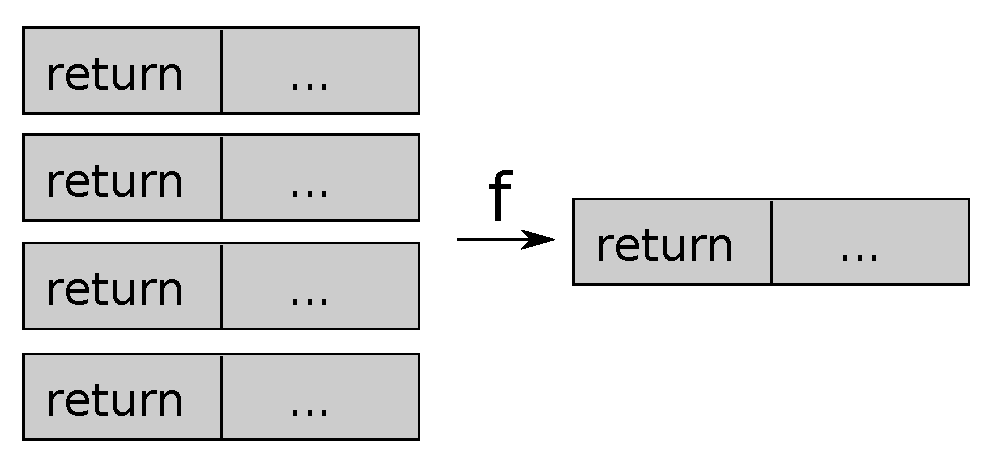
\includegraphics[height=100px]{purity-preservation}

Ist nicht sichergestellt, dass sämtliche Elemente der Eingabeliste rein sind, kann man sich weiter überlegen, dass eine
Möglichkeit zur Verfügung steht, mit der man den reinen Inhalt des monadischen Werts extrahieren kann - ähnlich wie
die unsichere Funktion \texttt{unsafePerformIO}, die den reinen Wert aus einer IO-Monade extrahiert, nur eben für
andere Monaden und sicher.
Es ist ja vorstellbar, dass man nur am reinen Ergebnis einer Funktion $f$ interessiert ist, unabhängig von eventuellen anhaftenden
monadischen Effekten. Tatsächlich kann man unter bestimmten Voraussetzungen zeigen, dass man beliebige Effekte in der 
Eingabeliste ignorieren kann, wenn man nur am reinen Ergebnis interessiert ist.

Sei $f :: Monad\ m \Rightarrow [m\ Int] \rightarrow m\ Int$, sei $\kappa$ eine Monadeninstanz und sei $p :: \kappa\ a \rightarrow a$, d.h. $p$ ist die erwähnte Funktion, die den reinen Wert aus dem monadischen Kontext extrahiert.
Wenn folgende Aussagen gelten:

\begin{itemize}
\item $p \circ return_{\kappa} = id$
\item Für beliebige Typen $t, t'$ und beliebige $m :: k\ t, k :: t \rightarrow k t'$ gilt\\
$p (m\ {>>=}_{\kappa}\ k) = p\ (k\ (p\ m))$
\end{itemize}

dann liefert $p \circ f_{\kappa}$ das gleiche Eregbnis für beliebige Listen gleicher Länge, deren Elemente an jeweils gleicher Position
die gleichen p-Bilder haben, sprich: den gleichen reinen Anteil. Man kann $p \circ f_{\kappa}$ kann also auch erhalten durch
$g \circ (map\ p)$ für eine passende Funktion $g :: [Int] \rightarrow Int$ \cite{voigtlander}.

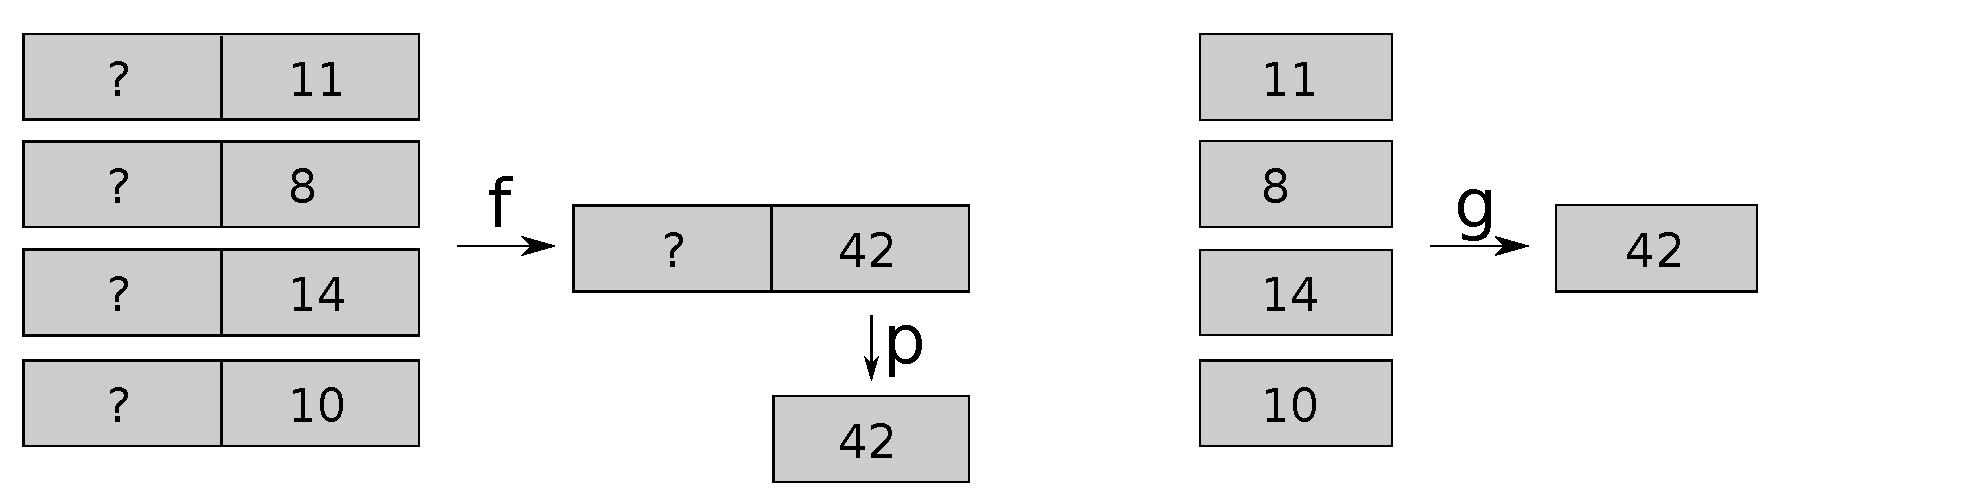
\includegraphics[height=100px]{safe-value-extraction}

Für diese Aussage werden keine Monadengesetze benötigt.

\newpage

\section{Die Bibliothek free-theorems} % TODO: diesen abschnitt weiter

In \cite{freetheorems} wird eine Implementierung vorgestellt, die die automatisierte Generierung von freien Theoremen aus
Haskell-Code ermöglicht und die Grundlage darstellt, auf die die vorliegende Arbeit aufbaut.
Sie erlaubt das Parsen von Haskell-Code, das Herausfiltern der entsprechenden Definitionen und deren relationale
Interpretation, um schließlich die freien Theoreme zu erzeugen.
Beigefügte Pretty printing Funktionen für Haskell-Syntax und Theoreme vereinfachen schließlich deren Darstellung.

Im folgenden Abschnitt wird erläutert, wie diese Bibliothek grundlegend aufgebaut ist, wobei auf jeden einzelnen Schritt genauer
eingegangen wird.

\subsection{Aufbau}

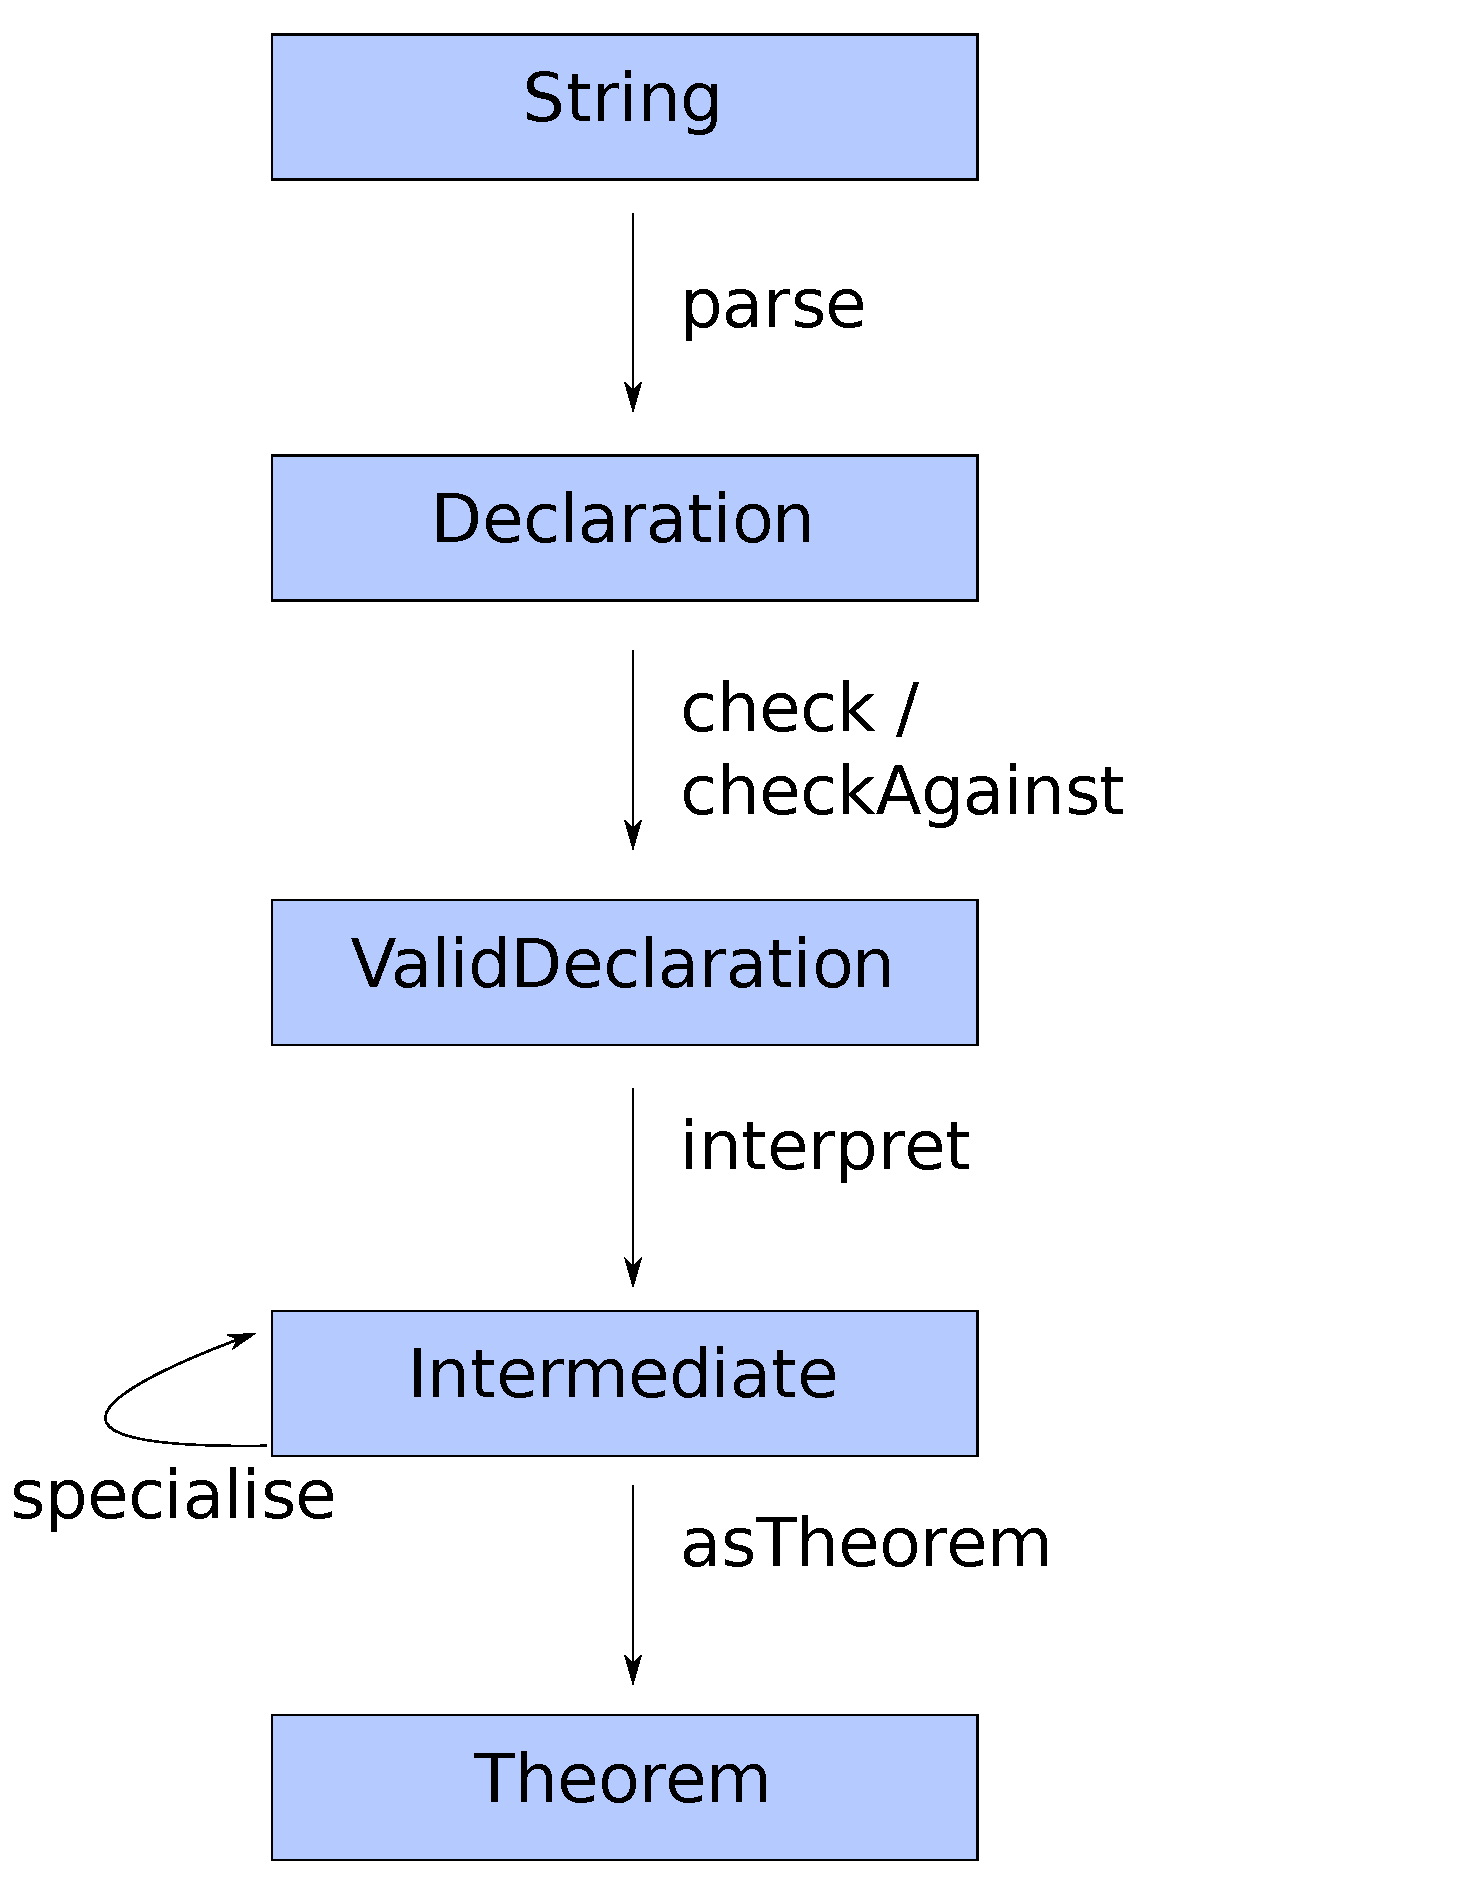
\includegraphics[height=250px]{overview-free-theorems}

\cite{freetheorems} gliedert die Bibliothek in drei grundsätzliche Teile: \todo{S. 53 Arbeit} Frontend, Core und Pretty printer. \todo{Abbildung zur Veranschaulichung?}
Zunächst werden im Frontend Parser bereitgestellt, um den Haskellcode aus einer Zeichenkette in eine passende Syntaxbaumstruktur umzuwandeln. Mithilfe einer check-Funktion
wird diese Datenstruktur auf Gültigkeit überprüft, insbesondere in Bezug auf spezielle Anforderungen, die an die Definitionen gestellt wird, um Theoreme zu generieren.

\texttt{interpret} ist dann schließlich die Funktion, die eine Signatur in Bezug auf die anderen Deklarationen in eine Zwischendarstellung \texttt{Intermediate} überträgt. Die
Funktion \texttt{asTheorem} entfaltet diese Darstellung \todo{``entfaltet''?} schließlich und überträgt sie in den Datentyp \texttt{Theorem}.

\subsection{Parser}

Neben dem Haskell 98 Parser, der keine \todo{Keine?} Spracherweiterungen zulässt, ist auch der Hsx Compiler gegeben, der die
komplette Sprache mitsamt Spracherweiterungen umsetzt. Hier ist anzumerken, dass das Paket free-theorems in seiner aktuellen Form
nicht mit dem aktuellen Haskell-Compiler kompatibel war und einige Anpassungen gemacht werden mussten. \todo{Evtl im Anhang Näheres?}
Intern nutzt free-theorems hier die Pakete \texttt{Language.Haskell.Parser} bzw. \texttt{Language.Haskell.Exts.Parser}, die an sich bereits voll funktionstüchtige Parser liefern.

Allerdings ist der komplette Sprachumfang sehr komplex und ein Arbeiten mit den Datenstrukturen, die von diesen genutzten Parsern generiert werden,
wird unnötig erschwert. Aus diesem Grund transformiert free-theorems diese Datenstruktur in eine eigene, vereinfachte Struktur namens BasicSyntax. In dieser Struktur
werden lediglich Typsignaturen festgehalten, Implementierungen werden vollkommen ignoriert, da sie für die Theoremgenerierung keine Rolle spielen.

\subsubsection{BasicSyntax}

Es soll hier zunächst an einigen Beispielen verdeutlicht werden, wie die BasicSyntax-Struktur definiert ist.

\inputminted[tabsize=2]{haskell}{ast.hs}

Listing \ref{lst:ast} zeigt die Datenstruktur am Beispiel der in der ersten Zeile angegebenen Definition. Die \texttt{parse}-Funktion des Parser-Moduls gibt eine Liste von Definitionen zurück, in diesem Beispiel nur ein Element mit dem Konstruktor \texttt{TypeSig}.

Natürlich ist man hauptsächlich an den Funktionssignaturen interessiert, da man aus diesen die Theoreme ableitet. Aber natürlich können diese Signaturen ihrerseits wiederum 
selbst definierte Datentypen oder auch Klasseneinschränkungen enthalten. Man kommt also nicht umhin, auch diese mit einzubeziehen und ebenfalls in der BasicSyntax vorzusehen.
Das Beispiel in Listing \ref{lst:ast-data} zeigt eine data-Deklaration.

\inputminted[tabsize=2]{haskell}{ast2.hs}

\subsection{check}
\label{sec:check}

Im zweiten Schritt wird die \texttt{check}-Funktion benutzt, um alle Deklarationen auf Gültigkeit zu überprüfen und die Liste der Deklaration zu filtern. Ungültige Deklarationen
werden unter Angabe einer Fehlermeldung aus der Liste entfernt \cite{freetheorems}.

Es ist zwar davon auszugehen, dass die Syntax des Programmes korrekt ist, da ansonsten der Haskell-Parser bereits im ersten Schritt einen Fehler gemeldet hätte, dennoch ist
dieser zweite Schritt nötig, um auch korrekte Semantik voraussetzen zu können \todo{wahrscheinlich falsch ausgedrückt} (da andernfalls auch für fehlerhafte Programme Theoreme generiert würden, was keinen Sinn macht).

Die check-Funktion untergliedert sich in lokale und globale Checks, wobei die lokalen Checks pro Definition durchgeführt werden, die globalen Checks beziehen sich auf die Gesamtheit aller Definitionen. Beispielsweise wird lokal überprüft, ob bei Deklarationen die freien Variablen auf der rechten Seite auf der linken Seite der Defintion deklariert sind, es wird sichergestellt
dass auf der linken Seite alle Variablennamen verschieden sind, primitive Datentypen nicht deklariert werden usw.

Unter die globalen Checks fällt z.B., dass zu einem Funktionsnamen nicht mehrere Deklarationen existieren, dass alle Typkonstruktoren die korrekte Anzahl an Parametern haben oder auch dass keine Kreise in der Typklassenhierarchie existieren \cite{freetheorems}.

Am Ende schließt \texttt{check} noch alle Typausdrücke, dh. bei frei vorkommenden Typvariablen werden entsprechende Typabstraktionen um den Ausdruck geschlossen. Das ist wichtig, da in der weiteren Implementierung davon ausgegangen wird, dass alle Typausdrücke geschlossen sind und entsprechende Typabstraktionen zu jeder implizit allquantifizierten Variable vorhanden sind.

Tabelle \ref{bla} zeigt eine Übersicht aller globalen Überprüfungen.

\begin{tabular}{| l | l |}
\hline
Name&Beschreibung\\
\hline
  checkUnique&\\
  checkArities&\\
  checkAcyclicTypeSynonyms&\\
  checkAcyclicTypeClasses&\\
  checkAllConsAndClassesDeclared&\\
\hline
\end{tabular}

\subsection{interpret}

Tatsächlich macht die \texttt{interpret}-Funktion nichts, was nicht schon bekannt ist \todo{Das heißt, wenn ich es denn schon geschrieben hätte}: Sie überführt die Funktionssignatur in eine
Relationsdarstellung, wobei sie Typvariablen neu generierte Relationsvariablen zuordnet. Um es mit der Aufteilung von \cite{freetheorems} auszudrücken, stellt sie den Übergang des Frontends zum Core dar, wo der interessante Arbeitsschritt ausgeführt wird.

Der Datentyp, der hier verwendet wird, heißt Immediate. Dieser Datentyp ist letztlich nur ein Container für eine Relation mit
dem repräsentierten Typausdruck, zusätzlichen (unendlichen) Listen von freien Variablennamen und sonstigen Zusatzinformationen.

\subsubsection{Relation}

Für die Darstellung als Relationen definiert free-theorems den Datentyp \texttt{Theorem}, der folgende Konstruktoren hat:

\todo{unvollständig. und evtl unnötig}

\begin{tabular}{| l | l | l |}
\hline
Konstruktor & Parameter & Entsprechung \\
\hline
RelVar & RelationVariable & $\alpha$ \\
FunVar & (Either Term Term) & ? \\
RelBasic & - & R \\
RelLift & TypeConstructor [Relation] & [R], etc. \\
RelFun & Relation Relation & $S \rightarrow T$ \\
RelFunLab & Relation Relation & $S \rightarrow T$ \\
RelAbs & RelationVariable (TypeExpression,  & $\forall R . F R$ \\
& TypeExpression) [Restriction] Relation & \\
FunAbs & ... & \\
\hline
\end{tabular}

Wie man sieht, fehlt noch ein Konstruktor für die neu eingeführte Variante, dass eine Typkonstruktorvariable auf Relationen
angewandt wird. Darauf wird in Abschnitt \ref{sec:erweiterung-typklassen} eingegangen.

\subsection{asTheorem}

Die \texttt{asTheorem}-Funktion stellt eine Datenstruktur des Typs \texttt{Intermediate} als Theorem dar. Tatsächlich passiert hier aber eine ganze Menge mehr als der Name
vermitteln mag. Das schrittweise Abrollen der Relationen stellt schließlich den entscheidenden Schritt dar, durch den man überhaupt auf
die Theoreme schließen kann.

\todo{Hier eventuell auch ein Beispiel?}

\subsection{Spezialisieren von Relationsvariablen zu Funktionen}

Ist das Theorem generiert, kann man nun die Funktionsrelation spezialisieren, um das Theorem zu vereinfachen. Aus einem
$A : S \leftrightarrow T$ wird also $\forall a : S \rightarrow T$

usw.

\subsection{simplify}

Schließlich bietet free-theorems noch die Möglichkeit, die generierten Theoreme zu vereinfachen, indem nach einigen typischen
Mustern gesucht wird, beispielsweise: Entfernen aller unbenutzten allquantifizierten Variablen, $\forall v. f v == g v \rightarrow f == g$ usw.

\subsection{Beispiel}

In den vorangegangenen Abschnitten wurde ein kurzer Umriss der Bibliothek free-theorems gegeben, die im Folgenden um
Typkonstruktorklassen erweitert werden soll. Bevor die benötigten Änderungen erläutert werden, soll hier zunächst ein
kompletter Durchlauf als Beispiel gegeben werden. Es werden sämtliche Daten betrachtetet, die auf dem Weg von einer
Eingabezeichnekette zur resultierenden Ausgabezeichenkette entstehen.

\todo{Grafik}

Wir bemühen wieder unser Beispiel aus der Einleitung:

\begin{minted}{haskell}
f :: [a] -> [a]
\end{minted}

Im ersten Schritt setzt man einen bereitgestellten Parser ein, um diesen Haskell-Code in den bibliotheksinternen, vereinfachten
Syntaxbaum \texttt{BasicSyntax} zu parsen. Die \texttt{parse}-Funktion gibt genaugenommen eine Liste von \texttt{Declaration}s, also Deklarationen. Dabei handelt es sich um alle Toplevel-Deklarationen, die eine Rolle spielen, also Funktionssignaturen,
Datentypdeklarationen und Klassendeklarationen.

\begin{minted}{haskell}
...
\end{minted}

Hier wurde die Darstellung ein wenig vereinfacht, um das Verständnis zu erleichtern. Zu beachten ist aber, dass sämtliche
Funktionsimplementierungen wegfallen. Sie spielen für die Generierung freier Theoreme keine Rolle, das bedeutet aber auch,
dass free-theorems keine Fehlerprüfungen im Implementierungsteil durchführt. Die Bibliothek kann ohne Auftreten von Fehlern
durchlaufen, selbst der zu einer Funktionssignatur gehörige Code Fehler enthält.

Jetzt, da die \texttt{BasicSyntax} der Beispielfunktion vorhanden ist, muss \texttt{check} aufgerufen werden, um Fehler
zu entdecken. Ein Aufruf macht aus der Liste von \texttt{Declaration}s eine Liste von \texttt{ValidDeclaration}s. Tatsächlich
enthält diese Datenstruktur lediglich ein zusätzliches Feld \texttt{isStrictDeclaration}, das anzeigt, ob die entsprechende
Deklaration strikte Elemente enthält oder von diesen abhängt.

Um genau zu sein, ist der Ergebnistyp von \texttt{check} monadisch, es werden per Writer-Monade Fehlermeldungen
generiert, falls Fehler auftreten. Es ist noch anzumerken, dass \texttt{check} auch beim Auftreten von Fehlern eine Liste
von Deklarationen zurückgibt. Lediglich die Deklarationen, die Fehler enthalten, werden weggelassen; das bedeutet, dass
unter Umständen Theoreme generiert werden können, wenn nur Fehler auftreten, die keine Auswirkung auf das zu generierende
Theorem haben.

\begin{minted}{haskell}
...
\end{minted}

An dieser Stelle haben wir eine Liste gültiger Deklarationen, und wir haben eine Liste eventell aufgetretener Fehler. Um nun
freie Theoreme zu einer Typsignatur zu generieren, wird zunächst einmal eine Typsignatur benötigt. free-theorems bietet die
Funktion \texttt{filterTypeSignatures}, um Typsignaturen aus einer Liste von \texttt{ValidSignature}s herauszufiltern, was in
unserem Beispiel keinen Unterschied macht, weil es lediglich aus einer Typsignatur besteht.

Jetzt können wir \texttt{interpret} verwenden, um zu unserer \texttt{ValidSignature} unter Verwendung der übrigen
\texttt{Declaration}s die Relationaldarstellung unsereres Datentyps

\section{Erweiterung um Typklassen und -konstruktoren}
\label{sec:erweiterung-typklassen}

In diesem Abschnitt soll erläutert werden, welche Änderungen an free-theorems vorgenommen werden müssen, um auch Typklassen und Typkonstruktoren miteinzubeziehen. In
Abschnitt 

usw.

\subsection{Erweiterungen der BasicSyntax}

Da Typvariablenapplikation in \cite{freetheorems} nicht vorgesehen ist, musste ein solches Konstrukt in die BasicSyntax-Struktur eingefügt werden. Hierbei ist zu beachten: Die Applikation
von Standardtypkonstruktoren, beispielsweise \texttt{[a]} für Listen, ist sehr wohl vorgesehen und wird in der BasicSyntax durch \texttt{TypeCon} im Datentyp \texttt{TypeExpression} dargestellt. \todo{Wahrscheinlich viel zu speziell} Diese Standardtypkonstruktoren werden in diesem Zusammenhang aber als Sonderfälle betrachtet \ref{sec:freie-theoreme}, um das System wirklich um eigene Typklassen zu erweitern, muss es auch möglich sein, Typkonstruktorvariablen auf Typen anzuwenden.

Die Erweiterung der BasicSyntax sieht hier so aus, dass ein neuer Konstruktor \texttt{TypeVarApp} zum Datentypen \texttt{TypeExpression} hinzugefügt wird. In Listing \ref{lst:typevarapp} ist ein Beispiel zu sehen.

\inputminted[tabsize=2]{haskell}{typevarapp.hs}

Abgesehen vom offensichtlichen Problem, dass dieser Konstruktor bei der Theoremgenerierung zu Fehlern beim Pattern Matching oder zumindest zu unerwünschtem Verhalten führt,
ist auch zu beachten, dass die in Abschnitt \ref{sec:check} erwähnte \texttt{check}-Funktion entsprechend angepasst wird.

\subsection{Erweiterung von Relation}

Da eine neue Relationskonstruktion eingeführt wird, muss auch der entsprechende Datentyp angepasst werden.

\subsection{Erweiterung von check}

Da in der ursprünglichen Version von free-theorems Typkonstruktorvariablen nicht gestattet waren, konnten einige
Fehlerüberprüfungen eingespart werden. Erlaubt man Typkonstruktorvariablen, muss man zusätzliche Fehlerfälle abdecken,
die auftreten können. Betrachten wir das folgende Beispiel:

\begin{minted}{haskell}
test :: Functor f => f a -> f
\end{minted}

Hierbei handelt es sich nicht um eine korrekte Haskell-Typsignatur: Die Variable f wird als Functor eingeführt und in der Signatur
einmal mit einem Parameter, einmal ohne Parameter aufgerufen. Selbst wenn man die Deklaration von Functor außer Acht lässt,
kann man deutlich sehen, dass eine der beiden Vorkommen von \texttt{f} fehlerhaft ist. \texttt{f} erwartet entweder einen
oder gar keinen Parameter, unterschiedliche Parameterzahlen sind nicht gestattet.

Da Functor bekannt ist, kann man einfach die Deklaration dieser Klasse betrachten:

\begin{minted}{haskell}
class Functor f where
   fmap :: (a -> b) -> f a -> f b
\end{minted}

Anhand der Deklaration der Klassenfunktionen kann man nun sehen, dass die Variable \texttt{f} stets auf einen einzelnen 
Parameter angewandt wird, das heißt, man kann bei allen Vorkommen der Klasse Functor davon ausgehen, dass diese
auf genau einen Parameter appliziert werden müssen. Natürlich kommt hier eine weitere Überprüfung ins Spiel: Es muss
sichergestellt werden, dass die Klassenvariable - in diesem Fall f - in sämtlichen Klassenfunktionen mit der gleichen Anzahl an
Parametern verwendet werden.

Die Überprüfung innerhalb einer Klasse auf gleiche Arität aller Vorkommen der Klassenvariable ist eine lokale Überprüfung -
es wird stets nur die Klassendeklaration benötigt, ein globaler Kontext muss nicht bekannt sein. Möchte man überprüfen,
ob Typkonstruktorvariablen in beliebigen Deklarationen die korrekte Anzahl an Parametern haben, dann muss man den
globalen Kontext betrachten: Die Deklaration der Klasse muss in Betracht gezogen werden.

Eine Besonderheit ist hierbei auch, dass eine Typvariable auf mehrere Klassen gleichzeitig eingeschränkt werden kann. So ist
das folgende Beispiel legitimer Haksell-Code:

\begin{minted}{haskell}
test :: (SomeClass1 f, SomeClass2 f) => f a -> f b
\end{minted}

Man muss also zusätzlich sicherstellen, dass alle Klassen, die für die gleichen Variablen angegeben sind, die gleiche Anzahl an
Parametern erwarten.

\section{Striktheit und Rekursion}

Bisher wurde eine Wahrheit größtenteils ignoriert: Die bisher generierten freien Theoreme sind nur unter ganz bestimmten
Bedingungen gültig. Beim Beispiel \texttt{$test :: [a] \rightarrow [a]$} wurde behauptet, dass die Funktion \texttt{test}
lediglich Ausdrücke aus der Eingabeliste in der Ausgabeliste weiderverwenden könne. Tatsächlich entspricht das nicht ganz der
Wahrheit, denn in Haskell ist zum Beispiel auch denkbar, dass $\bot$ (\textit{bottom}) zurückgegeben wird, beispielsweise
durch Nichtterminierung oder einen Laufzeitfehler.

free-theorems definiert verschiedene Untermengen der Programmiersprache Haskell, zu denen sich unterschiedlich komplexe
Theoreme generieren lassen. Ein Faktor, der nämlich Probleme bereiten kann, ist der Fixpunktoperator.
Die Bilbiothek definiert drei Untermengen:

\begin{itemize}
   \item BasicSubset
   \item SubsetWithFix
   \item SubsetWithSeq
\end{itemize}

Die erste Untermenge, BasicSubset, entspricht dem Girard-Reynoldschen Lambda-Kalkül \cite{bla}, erweitert um Datentypen und
Typklassen \cite{freetheorems}. Insbesondere sind aber keine undefinierten Werte erlaubt, die zum Beispiel durch Nichtterminierung,
Division durch Null oder Pattern Matching Fehler auftreten.
Das ändert sich in SubsetWithFix. Hier ist zusätzlich der Fixpunktoperator \textit{fix} verfügbar, und es müssen folglich undefinierte
Werte erlaubt werden. Was noch fehlt, ist die \textit{seq}-Funktion sowie Striktheits-Flags. Letztere können bei selbstdefinierten
Datentypen an die einzelnen Untertypen \todo{Richtige Bezeichnung für einzelne "Parameter" eines Datentyps?} annotiert werden,
um eine strikte Auswertung zu erzwingen.
Die Untermenge SubsetWithSeq ermöglicht schließlich die zuletzt genannten Aspekte: Es wird Striktheit durch \textit{seq}
eingeführt, dadurch sind dann auch Striktheitsannotationen in Datentypen möglich.

Es wird noch eine weitere Unterscheidung eingeführt: Zu SubsetWithFix und SubsetWithSeq kann noch unterschieden werden,
ob Gleichungs- oder Ungleichungsresultate gewünscht sind. \todo{equational and inequational results - bessere Übersetzung?}
Daraus ergeben sich insgesamt fünf Varianten, für die \cite{freetheorems} die folgende Schreibweise einführt, wobei $M$ die Menge
der verfügbaren \textit{Modelle} ist:

\begin{align}
M = \{(basic, =), (fix, =), (fix, \sqsubseteq), (seq, =), (seq, \sqsubseteq)\}
\end{align}

\section{Zusammenfassung}

\section{Ausblick}

\bibliography{masterarbeit}
\bibliographystyle{plain}

\end{document}
